\documentclass[a4paper,12pt]{article} 
\usepackage[a4paper,  fancysections,  titlepage]{polytechnique}
\usepackage[english]{babel}
\usepackage[T1]{fontenc}
\usepackage{blindtext}
\usepackage[hidelinks]{hyperref}
\usepackage{amsmath, amssymb}
\usepackage{subfigure}
\usepackage{graphicx}
\usepackage{tabularx,ragged2e,booktabs,caption}
\usepackage{hyperref}
\usepackage{dsfont}

\author{Xuan WANG}
\date{\today}
\title{Decarbonization of the maritime industry through deceleration}
\subtitle{Site Web of the project: \url{https://github.com/GearlessJohn/speed-reduction}}%
\logo{typographix}




\begin{document}

\maketitle

\newpage
\thispagestyle{empty}
\section*{Acknowledgements}

Before delving into the details of this professional experience, it seems appropriate to begin this internship report by expressing my gratitude to those who have taught me a great deal during this internship, and even to those who have graciously made this experience highly beneficial.\\

I would like to extend my sincere thanks to Ms.~Kristelle PILOT, my internship tutor who trained and guided me throughout this professional experience with great patience and amiability.\\

I am also grateful to Mr.~Pascal GIBART, the project manager, and Mr.~René AÏD, professor of economics at the University of Paris-Dauphine and lecturer at Ecole Polytechnique.
Their empathy, professionalism and extensive knowledge have consistently made the course of this training enjoyable.\\

I wish to express my thanks to Mr.~Thibaud ESCOFFIER, Ms.~Emilie SANCHEZ, Mr.~Eric PETIT, the shipping team of Crédit Agricole who have patiently provided me with technical support and information in the field of maritime transport.
To Ms.~Alix MATHIEU, my second tutor, and Mr.~Antoine CURTY, quantitative analyst, I want to say thank you for the material support and IT assistance.\\

Finally, I wish to express my gratitude to Mr.~Samy KARA MOSLI, the research internship supervisor, and Mr.~Nizar TOUZI, professor of mathematics at Ecole Polytechnique.
It is thanks to your attention and assistance that this work could be realized.




\newpage
\thispagestyle{empty}
\tableofcontents


\renewcommand{\thepage}{\arabic{page}}

\newpage
\setcounter{page}{1}
\section{Introduction}

% Motivate and abstractly describe the problem you are addressing and how you are
% addressing it. What is the problem? Why is it important? What is your basic approach? A
% short discussion of how it fits into related work in the area is also desirable. Summarize the
% basic results and conclusions that you will present
\subsection{Background}
Maritime shipping, which facilitates approximately 90\% of global commercial trade due to its robust capacity, cost-effectiveness, and notable safety record, has been placed in the spotlight amid global focus on sustainable development and environmental conservation.
Regrettably, the industry is a major emitter of pollutants, with significant impacts seen in high-traffic areas like ports and dense shipping routes.
Research by the International Maritime Organization (IMO) shows an increase in the industry's contribution to global greenhouse gas emissions (GHG), from 2.76\% to 2.89\% between 2012 and 2018.\\

Additionnal, forecasts from the IMO (2020) estimate an alarming 50\% increase in cabon dioxide (CO2) emissions from the shipping industry by 2050 when compared to the 2018 baseline if no measures are taken.
These sobering figures underline the urgency of the need to improve the maritime sector's environmental footprint and have been a catalyst for scientific research into the field of green shipping. Also, parteners involved in the maritime field are seeking supporting the maritime sector to achieve the blue economy concept.\\

I am currently working on the MQP (Quantitative Portfolio Models) in the Risk \& Permanent Control (RPC) department at Crédit Agricole.
Crédit Agricole Corporate and Investment Bank (CA-CIB) is a subsidiary of Crédit Agricole, one of the largest banking groups in the world.
Headquartered in France, Crédit Agricole CIB specializes in corporate and investment banking.
It offers an array of services, including structured finance, commercial banking, and international trade and transaction banking, catering to a diverse range of clients including corporates, financial institutions, sovereigns, and large multinationals.\\

In pariticular, Crédit Agricole was one of the funding signatories of the Poseidon Principles.
The Poseidon Principles are a framework established in 2019 to assess and disclose the climate alignment of ship finance portfolios.
Their main function is to align ship financing with the International Maritime Organization's greenhouse gas reduction targets, promoting a transition to a more sustainable maritime industry.
The principles require financial institutions to annually measure and disclose the carbon intensity of their shipping portfolios, collaborate with clients to develop decarbonization strategies, and transparently report their climate alignment scores and progress.
The Poseidon Principles have gained traction within the industry, with major signatories including leading international banks such as Citi, Societe Generale, ABN AMRO, BNP Paribas, DNB, and Crédit Agricole, and maritime lenders committed to driving decarbonization efforts in the shipping sector.
This aligns with the bank's broader commitment to environmental sustainability and responsible business practices. By adhering to the Poseidon Principles, Crédit Agricole CIB is committed to financing maritime projects that align with necessary climate goals.
This involves assessing the climate alignment of shipping portfolios, with an aim to enhance methodologies and strategies that drive decarbonization and sustainability in the shipping sector.
Therefore, \textbf{the main objective of my internship} is to build a model capable of calculating the expected speed of different vessels and the corresponding environmental impact, based on available market information, key data on ship navigation (annual range, fuel consumption, CO2 emissions, etc.) provided by Poseidon Principle and internal financial data from Credit Agricole CIB, as well as future forecasts.\\

On the other hand, in 2018, IMO published several strategies for the reduction of GHG emissions with the goal of reducing them by at least 40\% by 2030 compared to 2008 levels.
These include, but are not limited to, improving ship design, utilizing cleaner fuels, adopting energy-efficient equipment, and implementing voyage optimization.\\

\textbf{Improved Ship Design}: One strategy involves making modifications in the design of new vessels to make them more energy efficient.
This could include the introduction of new hull designs, the use of lightweight materials, and the implementation of energy-saving devices.
However, the effectiveness of these methods can be quite variable and depends heavily on factors such as ship type and operating conditions.
Also, such changes primarily affect new ships, leaving a large existing fleet unaffected.\\

\textbf{Cleaner Fuels}: The transition to cleaner fuels, such as Liquefied Natural Gas (LNG), biofuels, or hydrogen, can also reduce GHG emissions
However, these fuel sources are not without their problems. For example, the use of LNG can lead to methane slip, a potent greenhouse gas.
Biofuels can have sustainability issues, and hydrogen, while promising, requires significant infrastructure development and poses storage and safety challenges.\\

\textbf{Energy-efficient Equipment}: The use of energy-efficient equipment, such as more efficient engines or waste heat recovery systems, can contribute to lower emissions. However, this requires substantial capital investments and does not always guarantee consistent results due to the variability in operational conditions.
Moreover, these measures have only a limited effect on reducing GHG emissions (typically less than 10\%), which is far from the IMO's 40\% target.\\

\textbf{Voyage Optimization}: Voyage optimization includes measures such as weather routing and just-in-time arrival. While these methods can yield fuel savings, their effectiveness heavily depends on external factors like weather conditions and port operations, making the results less predictable.\\

In comparison, \textbf{speed reduction}, or "slow steaming," is a direct and reliable method for reducing fuel consumption and thus GHG emissions.
It can be implemented immediately across the global fleet, both old and new, without the need for significant capital investment.
Its effects are also highly predictable: as a rule of thumb, halving a ship's speed can reduce fuel consumption by more than three-quarters.
Therefore, speed reduction is often considered one of the most effective and reliable strategies for reducing GHG emissions in the maritime sector.\\

\subsection{Reduction of speed}
As a more intelligent and effective way of controlling the speed of different ships, the IMO has introduced the Carbon Intensity Indicator (CII) policy.
The CII calculates a ship's carbon intensity by dividing its annual CO2 emissions (measured in tonnes) by the vessel's transport capacity (deadweight tonnage, DWT) and the distance travelled. Therefore, the CII is directly influenced by a ship's speed - slower speeds mean lower fuel consumption and fewer CO2 emissions.\\

Each year, a ship's CII rating is compared to scheme set by the IMO, and the ship is rated from A to E, with A being the best performance and E the worst.
Ships rated D for three consecutive years or E for one year are subject to a review and may need to submit a corrective action plan and wait for the validation.\\

The CII incentivizes speed reduction more subtly and flexibly than a simple speed limit. Unlike a speed limit, the CII allows for variations in operational circumstances.
For instance, in conditions of bad weather or when higher speeds are required for safety reasons, ships can increase their speed without breaching regulations, providing they manage their speeds at other times to maintain a favorable CII rating over the year.\\

The main focus of this report will be on estimating the extent of speed reduction due to the CII policy and a potential carbon tax.
While speed reduction is a simple and effective means to reduce emissions, it also decreases the transport capacity of the global fleet, leading to an increased demand for new, more efficient ships.
It is essential to take into account the GHG emissions produced in the construction of these new vessels.
These emissions in construction phase can be significant and must be factored into a full lifecycle assessment of emissions from the shipping industry.\\

Ultimately, the most effective strategy will involve a combination of speed reduction, fleet renewal, and other measures, taking into account both operational and shipbuilding emissions.
This report aims to shed light on these complex interactions and provide more effective policy making for the decarbonization of the shipping industry.

% INCLUDE: results and conclusions

\newpage
\section{Theory}

\subsection{Definition of the problem}
% Precisely define the problem you are addressing. Elaborate on why this is an interesting and
% important problem.
\subsubsection{Current Policies}
The \textit{Global Emission Control} model aims to quantitatively evaluate the impact of CII and carbon tax on vessels' navigation speeds, and consequently on GHG emissions.
The imposition of CII limits and carbon tax policies is expected to compel the majority of maritime vessels to reduce their operational speed in an effort to optimize profit margins.
On the same time, fleet operators will likely need to order new vessels from shipyards to compensate for diminished transport capacity.
Inevitably, the construction of theses new vessels will contribute to greenhouse gas (GHG) emissions.\\

Furthermore, the maritime transport market will face a substantial supply reduction due to a global declartion of vessels and the fact that the construction of new vessels averages as two-year timeline.
Consequently, we can anticipate an extended period of increasing freight rates.
This translated into greater profit per voyage, which, in turn, allows vessels initially categorized with superior CII classifications (A) to incrementally increase their speed up to the regulatory limit (C or D) to maximize their profitability through increased trip frequency.
However, this acceleration will also result in an uptick in GHG emissions.\\

Thus, the ultimate question to be addressed is: \textbf{Will GHG emission decrease in the era of global maritime transport deceleration, and if so, to what extent?}\\

There are four primary stages:
\begin{itemize}
	\item Step 1: Annual profit optimization for one single vessel
	\item Step 2: 4-year profit optimization for one single vessel with CII limits
	\item Step 3: 4-year profit optimization for the fleet with construction of new vessel
	\item Step 4: Grouped profit optimization with a common price determined by speed distribution \\
\end{itemize}

In the stage of annual profit analysis, the optimal speed of a maritime vessel will be determined under the given conditions such as fuel prices, freight rates, carbon tax rates, and operation costs.
The investigation will initiate with the reconciliation of a singular voyage.
However, it should be noted that the duration of a vessel's journey is significantly affected by its velocity.
If a ship's total voyage time in a year doesn't change, say 300 days, the increase in speed will allow a greater number of voyages to be made.
However, the reality is that as the number of voyages increases, more time will be spent loading and unloading at ports, which will ultimately reduce total voyage time in this year.
Last year, for example, a container ship spent 300 days (10 trips) at sea, 30 days loading and unloading in ports, 30 days waiting to enter ports and 5 days on maintenance.
If this container ship decides to speed up by 50\%, it won't be able to make 15 trips.
Because more time will be spent in ports and waiting, and the voyage time will be less than 300 days. \\

Upon acquiring the annual profit-speed curve, the constraints posed by the Carbon Intensity Indicator (CII) limits can be incorporated into the analysis.
The International Maritime Organization (IMO) stipulates that all vessels maintaining a CII rating of Class D for a duration exceeding or equal to three years, or a Class E for more than or equal to one year, are required to withdraw from the market.
Subsequently, these vessels must formulate and implement necessary remedial action plans, encompassing initiatives such as engine modifications and the utilization of low-carbon emission fuel, among others.
These measures are designed to demonstrate their capacity to comply with the Class C requirements and successfully undergo verification procedures, thereby facilitating their re-entry into the maritime market.
In reality, the cost of low-carbon emission fuels such as LNG and ammonia is too expensive to be affordable for most fleets.
Additionnally, engine modifications has limited impact on improving a vessel's CII score.
Therefore, in this model, we assume that if a vessel is forced to withdraw from the market, it cannot return.\\

Now, the fleet can optimize the speed of all vessels in compliance with CII regulations.
To meet demand after the speed reduction due to the carbon tax and CII limits, the fleet needs to order new vessels.
The main principle is this: if a fleet of 50 container ships loses, for example, 10\% of transport capacity due to speed reduction, it will order 10\% of 50, which equals 5, new container ships.
However, if the optimal choice is to accelerate, the fleet will not sell or destroy any vessel.\\

Finally, it is essential to consider the impact of the equilibrium between supply and demand on freight rates.
One fundamental premise in our analysis of the maritime transport market is the relative stability of demand.
Consequently, the key variable to be considered is the supply, which is directly proportional to the speed of the vessels. We will conduct this equilibrium analysis independently, implying that the speed alterations of a particular vessel category have no bearing on the markets of other vessel categories.
The primary objectives of this stage is to ascertain the elasticity of freight rates with respect to supply under the assumption of a fixed demand.\\

\subsubsection{Future projection}
The Global Emission Control model above is a model designed to investigate the impact of current policies (CII and carbon tax) on ship speed and carbon emissions.
However, the current CII policy will only be in place until 2026.
Under the current policy, for each category of vessel, its scoring criteria for 2023-2026 can be calculated in advance.
It is as if for a student, he would know in 2023 that the A standard for that year is 16/20, the next year is 16.2/20, and so on.\\

For new policies in 2027 and beyond, IMO will need to consider further in light of the effect of emissions reductions in the global fleet in 2023-2026.
As part of the task of this internship is to inform policy decisions, we consider a new possibility: to phase out vessels based on a proportion rather than a fixed score, for example the top 5\% of CII scores each year.
This would be like a school eliminating the 5\% of the lowest achievers each year.
To investigate the speed strategy of vessels in this case, Mr.~René AÏD and Mr.~Nizar TOUZI jointly propose a new model based on Mean-field. In this paper, it is referred to as \textit{Competiton} model in order to distinguish it from the Global Emission Control model.

\subsection{Global Emission Control Model}
% Describe in reasonable detail the methods the paper considers. A pseudocode description of
% the algorithm you are using is frequently useful. Trace through a concrete example, showing
% how the method processes this example. The example should be complex enough to
% illustrate all of the important aspects of the problem but simple enough to be easily
% understood. If possible, an intuitively meaningful example is better than one with
% meaningless symbols.
\subsubsection{Step 1: Annual Profit Optimization (one vessel)}

The process of annual profit optimization will be segmented into two components: first, the calculation of profit per voyage as a function of speed, and second, the calculation of the number of voyages as a function of speed.
The ultimate annual profit will the derived as the product of these two elements.\\

In this model, we assign a fixed route to each vessel. The route information includes voyage distance $D$, loading rate $LR$, and freight revenue $FR$ (USD/unit delivered).

The revenue and expenses of a route mainly include:
\begin{enumerate}
	\item Fuel costs
	\item Operating expenses (crew salaries, loading and unloading costs, etc.)
	\item Carbon tax costs
	\item Freight revenue
\end{enumerate}

According to physical calculations and actual vessel data, the fuel cost per unit distance, or fuel consumption, is cubically related to the speed of the vessel.
However, this relationship only holds when the speed is greater than about 13 knots, and when the speed is lower than 13 knots, we can approximate that the fuel consumption is proportional to the quadratic side of the speed.

\begin{equation}
	\label{eq:fuel_consumption}
	Fc^i(v) =
	\left\{
	\begin{aligned}
		\frac{Fc^i_{ini}}{D_{ini}} \cdot D \cdot (\frac{v}{v_{ini}})^3, \quad if \, v_{ini} > 13 \\
		\frac{Fc^i_{ini}}{D_{ini}} \cdot D \cdot (\frac{v}{v_{ini}})^2 \quad if \, v_{ini} \leq 13
	\end{aligned}
	\right.
\end{equation}

$Fc^i_{ini}$, $D_{ini}$ and $v_{ini}$ are the annual fuel consumption, annual voyage distance and annual average speed for 2021, respectively, provided by Credit Agricole CIB.
And $i$ represents different types of fuels, including Heavy Fuel Oil (HFO), Light Fuel Oil (LFO), Diesel and Liquefied Natural Gas (LNG). D is the distance of a certain route, and v is the actual voyage speed.
In reality, most container ships have an average annual speed between 15-17 knots, while bulk carriers have an annual average speed between 10-12.5 knots.
Thus, the above formula can be well applied to different situations.\\

The final fuel cost is the fuel consumption of each category multiplied by the fuel price of each category:

\begin{equation}
	\label{eq:fuel_cost}
	FC(v, FP) = \sum_i FP_i \cdot Fc^i(v)
\end{equation}

where $FC(v)$ is the fuel cost of a vessel for a given route at speed v and $FP_i$ is the market price of fuel type $i$. Unlike cars, ships usually have a choice of fuels. For example, most LNG carriers can run on both LNG and LFO.\\

Emissions of GHG are directly proportional to fuel consumption.
Similar to equation (\ref{eq:fuel_consumption}), we can obtain the carbon tax for a voyage as:

\begin{equation}
	\label{eq:emission}
	CT(v) =
	\left\{
	\begin{aligned}
		\frac{EM_{ini}}{D_{ini}} \cdot D \cdot (\frac{v}{v_{ini}})^3 \cdot CR, \quad if \, v_{ini} > 13 \\
		\frac{EM_{ini}}{D_{ini}} \cdot D \cdot (\frac{v}{v_{ini}})^2 \cdot CR, \quad if \, v_{ini} \leq 13
	\end{aligned}
	\right.
\end{equation}

$CT(v)$ is the carbon tax cost of the route at speed $v$, $EM_{ini}$ is the annual $CO_2$ emissions of the vessel in 2021, and $CR$ is the carbon tax rate (reference value of \$94 per ton of $CO_2$ emissions in 2023).\\

For operating cost OC, the fleet did not provide specific data due to confidentiality reasons.
But according to various \href{https://transportgeography.org/contents/chapter5/maritime-transportation/containerships-operating-costs-panamax-post-panamax/}{[reports]}, we can know that in the absence of carbon tax, the fuel cost of a ship generally accounts for 45\%-50\% of its total cost.
In this model, we assume that the operating cost of a single voyage is independent of speed.
In 2021 the carbon tax does not cover the shipping sector, and we assume that freight costs are 50\% of total costs in 2021, then for selected routes:

\begin{equation}
	\label{eq:operation_cost}
	OC = FC(v_{ini})
\end{equation}

For a vessel, it has four main types of time:
\begin{enumerate}
	\item Voyage time (180-260 days)
	\item Port time (20-120 days)
	\item Waiting time (30-90 days)
	\item IDLE time (10-60 days)
\end{enumerate}

Among them, voyage time is the time the ship sails; waiting time is the time the ship waits to enter the port; port time is the time the ship loads and unloads cargo in the port; idle time is the time the ship is inactive for various reasons.
The waiting time $WT$ and port time $PT$ are positively correlated with the number of voyages $N$.
Note that the voyage time is $VT$, and the time of year is $YT$ (365 * 24h). \\

The number of route sailing $N$ is the total sailing time $VT$ (hours) multiplied by the speed $v$ (knots = nautical miles / hours) divided by the distance of the route $D$ (nautical miles):
\begin{equation}
	\label{eq:vt}
	N(v) = \frac{VT(v) \cdot v }{D}
\end{equation}

For most vessels:
\begin{equation}
	\label{eq:ptwt0}
	WT_{ini}+PT_{ini} = 0.9 \cdot (YT-VT_{ini})
\end{equation}

$WT_{ini}$, $PT_{ini}$ and $VT_{ini}$ are the waiting time, port time and voyage time in 2021, respectively.
When the speed changes, the waiting time $WT$ and port time $PT$ are positively correlated with the number of voyages $N$, we have:
\begin{equation}
	\label{eq:ptwtv}
	WT(v)+PT(v) = \frac{N(v)}{N(v_{ini})} \cdot (WT_{ini} + PT_{ini})
\end{equation}

We assume that the time of the idle is essentially constant, so that the sum of the other three parts is constant:

\begin{equation}
	\label{eq:constant_sum1}
	WT_{ini}+PT_{ini}+VT_{ini} = WT(v)+PT(v)+VT(v)\\
\end{equation}

Bringing in equations (\ref{eq:ptwt0}) and \ref{eq:ptwtv}, we get:

\begin{equation}
	\label{eq:constant_sum2}
	0.9 \cdot (YT-VT_{ini})+VT_{ini} = \frac{N(v)}{N(v_{ini})} \cdot (0.9 \cdot (YT-VT_{ini}))+VT(v)\\
\end{equation}

Then bringing in equation (\ref{eq:vt}), we get:
\begin{equation}
	\label{eq:nv0}
	0.9 \cdot (YT-VT_{ini})+VT_{ini} = \frac{N(v)}{N(v_{ini})} \cdot (0.9 \cdot (YT-VT_{ini}))+\frac{N(v) \cdot D}{v}\\
\end{equation}

i.e.

\begin{equation}
	\label{eq:nv}
	N(v) = \dfrac{(0.9YT+0.1VT_{ini})}{(0.9(\frac{YT}{VT}-1)\frac{D}{v_{ini}}+\frac{D}{v})}
\end{equation}

Assuming limited speed variation does not affect the freight income ($FI$) from a voyage (e.g. a bulk carrier contract from Houston to Shanghai would typically have the same freight rate for a 40-55 day voyage). Then for one trip:

\begin{equation}
	\label{eq:FI}
	FI =  Capacity \cdot 95\% \cdot FR \
\end{equation}
where $FR$ is freight rate and 95\% is the average loading rate.\\

Finally we can get that the relationship between annual profit $AP$ and speed of a ship for a fixed route is:

\begin{equation}
	\label{eq:annual_profit}
	AP(v, FP, FR, CT) = (FI-FC(v, FP)-CT(v)-OC) \cdot N(v)
\end{equation}

where $FP$ is fuel price, and $CT$ is the carbon tax rate.


\subsubsection{Step 2: 4-year Profit Optimization (one vessel)}
The 4-year period refers to the 4 years from 2023 to 2026. The official implementation of the IMO CII restrictions will be in 2023.
Besides, the CII restriction policy (reduction factor) after 2026 is not yet available.
So we only consider this time period for now.\\

The difference between 4 years and 1 year of profit optimization for a ship is the IMO limit for CII.
IMO states that if a ship receives a D rating for 3 consecutive years or an E rating in a given year, then the ship needs to be taken off the market.
In this model, we do not consider the ship's plans for refit and fuel replacement to return to the market.
That is, once a ship does not comply with CII regulations, it needs to be permanently withdrawn from the market.\\

The formula for CII is:
\begin{equation}
	\label{eq:cii}
	CII_{atteined} = \frac{CO_2(g)}{Capacity(ton) \cdot Distance(nm)}
\end{equation}

$Capacity$ refers to the deadweight tonnage (DWT), which is the maximum cargo weight of the ship (not the actual cargo capacity);
$Distance$ is the distance travelled throughout the year;
and $CO2$ is the annual CO2 emission, which is obtained by multiplying the consumption of different fuels by their emission factors and summing them up.\\

For a vessel, its capacity is fixed and its CO2 emission per nautical mile is the product of its fuel consumption per nautical mile and the carbon intensity of the fuel used.
So, according to equation 1, we have:
\begin{equation}
	\label{eq:cii_model}
	CII(v) =
	\left\{
	\begin{aligned}
		CII_{ini}\cdot (\frac{v}{v_{ini}})^3, \quad if \, v_{ini} > 13 \\
		CII_{ini} \cdot (\frac{v}{v_{ini}})^2 \quad if \, v_{ini}\leq 13
	\end{aligned}
	\right.
\end{equation}

In addition, in order to calculate the optimal speed for 2023-2024, we need to estimate the fuel and freight prices for this period.
In this model, \textbf{we use a range of \href{https://www.cmegroup.com/markets/energy/refined-products/singapore-380cst-fuel-oil-platts-swap-futures.html}{[fuel futures prices]} and average them on an annual basis}.
Beyond that, \textbf{for calculations up to step 3, we assume that freight rates remain constant in 2023-2026}.\\


In the absence of CII restrictions, if we want to calculate the 2023-2026 optimal speed combination, we only need to calculate the optimal velocity for each year separately.
This is because the speed selection and profit of the previous year have no effect on the later year.
Assume that the original optional speed space for a ship is 13-19 knots.
We take a point every 0.1 knots of speed, and we have $\{13.0, 13.1 ... 19.0\}$ for a total of 61 points.
Then the domain of optimization without CII limits is $61 \cdot 4 = 244$ points.
But in the case of CII limits, the profit in a given year depends not only on the choice of speed in that year, but also on the choices of speed before.
For example, if a ship receives a three-year D rating in 2023-2025, it must withdraw from the market in 2026, regardless of the ship's originally planned 2026 speed.
If we take the classical greedy algorithm, i.e., we first calculate the optimal speed in 2023 to maximize the profit in 2023, and then use this as a basis to calculate the profit in 2024.
Then it is likely that one year will be accelerated to obtain an E rating in order to maximize this year's profit, thus forgoing profits for the following years.
Therefore, the greedy algorithm cannot produce an optimal solution.
In order to optimize the total profit, we must take into account the choices of speed of the 4 years jointly.
In this case, the domain of optimization becomes $\{13.0, 13.1, ..., 19.0\}^4$ containing $61^4 = 13 \,845 \,841$ points.\\



Denote $V = (v_0, v_1, v_2, v_3)$ as the choice of velocity for 2023-2026.
Also, for 2023-2026, note $FP=(FP_0, FP_1,FP_2,FP_3)$ as the fuel price, $FR=(FR_0,FR_1,FR_2,FR_3)$ as the freight rate, and $CT=(CT_0, CT_1, CT_2, CT_3)$ as the carbon tax rate.
In summary, the profits for 2023-2026 $P=P_0+P_1+P_2+P_3$ are:

\begin{align}
	\label{eq:P}
	P_0(V, FP, FR, CT ) & = AP_0                                                                                   \\
	P_1(V, FP, FR, CT ) & = AP_1 \mathds{1} _{CII_0 \neq E}                                                        \\
	P_2(V, FP, FR, CT ) & = AP_2 \mathds{1} _{E \notin {CII_0, CII_1}}                                             \\
	P_3(V, FP, FR, CT ) & = AP_3 \mathds{1} _{E \notin {CII_0, CII_1, CII_2}\,\&\, (CII_0, CII_1, CII_2)!=(D,D,D)}
\end{align}

where $AP$ is the annual profit function established in previous section:
\begin{equation}
	AP_i = AP(v_i, FP_i, FR_i, CT_i)
\end{equation}

In this model, each vessel can choose its speed based on the 2021 speed, plus or minus 3.0 knots.
The interval is 0.1 knots, yielding a total of 61 choices.
Ultimately we can obtain the optimal combination of speeds $V^\ast$ for a ship under the CII limit by using the following formula:
\begin{equation}
	\label{eq:vast}
	V^\ast = \operatorname*{argmax}_{V\in \{v_0-3.0, v_0-2.9, ..., v_0,...,v_0+3.0 \}^4} P(V, FP, FR, CT)
\end{equation}


The final domain of optimization will be a set of $61^4$ points.
And we cannot compute the optimal solution directly in reverse order.
Let's consider the optimization of profits in a reverse chronological order.
The sequence can be described as follows:

\begin{align*}
	v_3^\ast & = \operatorname*{argmax}_{v_3} (AP(v_3, FP_3, FR_3, CT_3))                                                                                                                                                    \\
	v_2^\ast & = \operatorname*{argmax}_{v_2}  (AP(v_2, FP_2, FR_2, CT_2)+AP_3^\ast \mathds{1} _{CII_2 \neq E} )                                                                                                             \\
	v_1^\ast & = \operatorname*{argmax}_{v_1}  (AP(v_1, FP_2, FR_2, CT_2)+(AP_3^\ast \mathds{1} _{CII_2 \neq E}+ AP_2^\ast )\mathds{1} _{CII_1 \neq E} )                                                                     \\
	v_0^\ast & = \operatorname*{argmax}_{v_1}  (AP(v_1, FP_2, FR_2, CT_2)+((AP_3^\ast \mathds{1} _{CII_2 \neq E \& (CII_{0,1,2}) \neq (D,D,D)}+ AP_2^\ast)\mathds{1} _{CII_1 \neq E} +AP_1^\ast )\mathds{1} _{CII_0 \neq E}) \\
\end{align*}

where $AP_i^\ast = AP(v_i^\ast, FP_i, FR_i, CT_i)$ and $CII_i$ is a function of $v_i$ as showed in equation (\ref{eq:cii_model}).\\

\begin{table}[h!]
	\centering
	\begin{tabular}{|c|c|c|c|}
		\hline
		      & C   & D   & E   \\
		\hline
		$P_4$ & 1   & 0.9 & 0.8 \\
		\hline
		$P_3$ & 1.1 & 1.5 & 1.3 \\
		\hline
		$P_2$ & 1.2 & 1.5 & 1.6 \\
		\hline
		$P_1$ & 2.5 & 3   & 3.2 \\
		\hline
	\end{tabular}
	\caption{Sample Profit Table}
	\label{tb:sample_profit}
\end{table}

The table (\ref{tb:sample_profit}) is a tabular representation of the profit margins based on different conditions.
We proceed by computing the maximum profit of year 4, where $P_4 = 1$ and $C_4 = C$. Subsequently, we obtain $P_3 = 1.5$ and $P_2 = 1.5$ with $C_3 = C_4 = D$. For the first year, the fleet is necessitated to choose a speed such that $C_1 = C$, if it aims to retain its entire profit from year 4. Consequently, $P_1$ escalates to 2.5, enabling the fleet to retain the profit of year 4. The cumulative profit totals to $1+1.5+1.5+2.5 = 6.5$. However, there might exist a superior choice, namely to decelerate in year 2 to enforce $C_2 = C$. Then, $P_2$ decreases to 1.2, but $P_1$ increases to 3, whilst retaining $P_4 = 1$. Consequently, the final total profit amounts to $1 + 1.5 + 1.3 + 3 = 6.8$.


\subsubsection{Step 3: Construction of new vessels}
The construction principle is very simple: compensate for the decrease in transport capacity caused by a reduction in speed.
We define annual transport capacity $AC$ of a vessel as the carrying $Capacity$ (unit of deadweight tonnage (DWT) or twenty-foot equivalent unit (TEU)) multiplied by the average speed $v$ and the annual voyage time $VT(v)$ at that speed.:
\begin{equation}
	\label{eq:AC}
	AC(v) = VT(v)  \cdot v \cdot Capacity
\end{equation}

The sample vessels provided by CA-CIB include 8 vessels of different categories (container ship, bulk carriers, tanker, gas carrier) and different sizes (Handysize, Panamax, etc.) under each category.
It is assumed that each ship is built independently of the other, since the purpose of each search is different and thus not interchangeable.
After obtaining the optimal speed for each year in the previous step, we can calculate the transport capacity gap $GAP$ for each year $i$ based on this speed:

\begin{equation}
	\label{eq:gap}
	GAP_{i} = max(1 - \frac{AC(v_i) \cdot Nmb(i)}{AC(v_0) \cdot Nmb_{ini}}, 0)
\end{equation}

where $Nmb(i)$ is the number of this kind of vessel in year i and $Nmb_{ini}$ is its initial number in 2021.\\

The $GAP$ will not be less than 0.
This is because the fleet will not destroy vessels when the acceleration of vessels in a given year results in a higher transportation capacity than the initial value of 2021.
The principles of construction are:
\begin{enumerate}
	\item Initial number of all types of ships is 1.
	\item The fleet will not destroy vessels.
	\item It takes 2 years for a ship to be delivered from the time the order is placed.
	\item For year $i$, if in $i+1$ year the fleet is about to receive $x$ new vessels, the new orders for that year are $max(GAP_i - x, 0)$.
	\item The cost of construction and GHG emissions are immediately credited to the year in which the order is placed.
\end{enumerate}


For example, if the gap of a ship is calculated to be [10\%, 12\%, 3\%, 5\%], then the number of such ships will be [1.00, 1.00, 1.10, 1.12].
The number of vessels in the first two of these years is unchanged, as it takes at least two years to build new vessels.
And although the gap in the second year is 12\%, the number of new orders in the second year is not 0.12, but $0.12-0.10=0.02$.
Since the fleet knew it was about to receive 0.10 new ships in the following year, there was no need to place an additional order for 0.12.\\

In particular, newly manufactured ships do not affect the calculations in step 2.
This is because in this model the newly built ships are not assumed to be more energy efficient or otherwise changed than the old ships.
Construction simply increases the number of vessels of a particular type in the fleet, and the whole calculation in step 2 depends only on vessel characteristics (load capacity, fuel consumption, type of vessel, fuel type, etc.) and market conditions.
Therefore, without taking into account the change in the number of vessels, i.e. the change in supply, for the change in the market price, the same strategy is simply used for the same type of vessel once the new one has entered the market.
Therefore, the calculations in step 2 do not need to be repeated.


\subsubsection{Step 4: Volatile freight rates}
In the previous section we considered the change in the number of ships under the fleet.
Now we need to consider the impact of the supply-demand balance on freight rates.
The model assumes that the supply of the ship market in 2021 is equal to the demand.
In order to evaluate the relationship between price and supply when demand remains constant, we collected global freight rate data from the Clarkson Index and China's export value for the years 2008-2023.
We consider China's export value to represent market demand and assume that market supply capacity remains unchanged in the short term (as the construction of new vessels requires time).
By conducting a linear regression on the two sequences formed from the annual percentage changes relative to the previous year for both variables, we determined that the elasticity of freight rates with respect to demand is 1.93.
We assume that from the equilibrium point where demand is equal to supply (say 10 and 10), the increase in demand (11 demand and 10 supply) has the same effect on the freight price as the decrease in the same quantity of supply (10 demand and 11 supply).
It is the difference between the two that matters.
Under this assumption, the elasticity of freight rates with respect to supply is -1.93.
This means that from the equilibrium point, for every 1\% reduction in supply with constant demand, freight rates rise by 1.93\%.\\

In addition to this, we assume that the markets for different categories of ships do not affect each other.
But different sizes of ships under the same category share the same freight price.
For a particular type of ships such as container ships, in year $i$, it has a freight price as:

\begin{equation}
	\label{eq:fr_mf}
	FR(i) = FR_{ini} \cdot \left (2.93 - 1.93 \cdot \frac{\sum_{j \in Container} AC_j(v_i) \cdot N_j(i)}{\sum_{j \in Container} AC_j(v_0) \cdot N_{j,ini}}\right )
\end{equation}


In the process of ensuring stable freight rate calculations, we employ the widely-recognized Expectation-Maximization (EM) algorithm, structured as follows:

\begin{enumerate}
	\item Initialization of all parameters is carried out, where the initial freight rate values for the period of 2023-2026 are set equal to the market price of 2023.
	\item \textbf{M}: Based on these initial prices, the fleet then makes decisions (equation (\ref{eq:vast})) concerning each ship's speed and the number of ships to be built, all in pursuit of total profit maximization.
	\item \textbf{E}: Subsequent to these decisions, freight rates for each type of vessel and for each year are recalculated based on equation (\ref{eq:fr_mf}).
	\item Repeat steps M and E until either a specified convergence condition is achieved, such as the average absolute change in speed being less than 0.1, or the maximum predetermined number of iterations has been reached.\\
\end{enumerate}


\subsubsection{Theoretical justification and guarantees}
% Provide here some formal theory justifying the correctness of the method. If it applies, state theoretical guarantees and provide a brief overview of the analysis.

\paragraph{Deterministic Solution up to Step 3:}

In the context of our model for calculating the optimal speed of global ships under policies such as CII and carbon taxes, it is important to highlight the deterministic nature of the calculations up to step 3.
Deterministic calculations refer to computations that produce the same results given the same inputs and conditions, without any element of randomness or uncertainty.\\

In our case, the calculations up to step 3 involve the determination of the optimal speed choice under the CII policy for 4 consecutive years with construction of new vessels.
These calculations are performed using discrete choices of speed, with a granularity of 61 values raised to the power of 4, resulting in a finite and discrete set of possible speed combinations.
Thus, the determination of the maximum profit and the corresponding optimal speed can be calculated with certainty.
By exhaustively evaluating all possible speed combinations within the defined range, the maximum profit and the corresponding optimal speed can be determined precisely.\\

\paragraph{Choice of EM Algorithm in Step 4:}

There are two key issues about EM algorithm:
\begin{itemize}
	\item In this model, each ship is not symmetric with respect to its price impact. Because a larger ship has a larger carrying tonnage, its acceleration and deceleration have a greater impact on price. As a result, the Mean-field model cannot be applied as it supposes that every player should be perfectly symmetric. While in the standard Mean-field model where we have a definite unique solution which is a fixed point, in this report, we cannot make directly use of these convergence properties.
	\item The EM procedure does not necessarily converge in this model. In other words, the maximum profit per ship will not have only an increasing trend. It is usually constantly fluctuating. For this reason, we need to limit the maximum number of iterations.
\end{itemize}

For the first problem, since the optimization space in this model is discrete and finite, for example, a market consisting of three container ships, all possible speed choices to maximize the total profit of the three ships are $61^{4*3} = 61^{12}$.
However, the computational overload makes it impossible to calculate all possibilities and find the optimal solution using a method similar to the one used in step 3.
We must therefore adopt certain heuristic algorithms.
In this model we have used the EM algorithm, not only because the principles of this algorithm are clear and relatively reliable, but also because it is the closest to real market changes compared to other algorithms such as neural networks.
That is, the market price changes and subsequently, after a delay, the major fleets adjust their supply capacity.
After a further delay, the market price adjusts to the previous change in supply to start the next cycle.\\

The fundamental reason for the second problem is that the entire shipping market is a negative feedback system.
That is, when fleets generally accelerate to increase supply, freight prices fall, which in turn causes fleets to slow down to reduce fuel costs and increase profits.
Conversely, when fleets generally slow down, demand outstrips supply in the market, freight rates rise and fleets choose to increase speed to increase the number of trips per year in order to maximize profits.
In fact, under some extreme initial conditions, the EM program can even go into oscillation. That is, the speed of the fleet keeps cycling between two modes, V1-V2-V1-V2, etc.
Also to solve this problem, the algorithm sets the maximum number of iterations.


\subsection{Competition Model}
In the Competition model, we focus on a two time-step model that pertains to the reduction of carbon emissions in the shipping industry.
The model revolves around a single decision variable, namely the speed of the vessel $u$.
In this model, the number of ships will no longer be based on a fleet, but on the whole shipping market, as it is needed to inform IMO decisions.
A number of simplifications and approximations are therefore required to reduce the computational effort and to make appropriate corrections to use the mean-field model.\\

In the beginning, we formulate the model within an N-player setting, and subsequently, we develop the Mean-field version. The model considers two distinct time points: $t = 0$ and $t = T$, where vessels are required to make decisions at $t = 0$.\\

Firstly, we assume that the relationship between the speed of the ship and the fuel consumption for one trip is essentially linear after successive decelerations starting in 2026. Ultimately, the cost for one year is:

\begin{equation}
	\label{eq:cost}
	c(u_i) = l u_i + \frac{1}{2 \gamma} u_i^2
\end{equation}

where the primary items are costs related to the number of voyages only (port charges, etc.) and the secondary items are those related to fuel consumption (e.g. fuel consumption, carbon tax).\\

And the freight price in the market is influenced by the speed of all ships.
Since we only consider the market for a particular ship type in this model (e.g. POST-PANAMAX type container ships), we can approximately ignore the difference in carrying capacity between different specific ship types (DWT 90000-110000t). In fact, there is no difference between all the vessels in this model, except for their carbon emission performance. Assuming that the speed of each ship has a symmetric effect on the market price, we have:

\begin{equation}
	\label{eq:price}
	p(u) = a - b \frac{1}{N}\sum_{i=1}^N u_i
\end{equation}

Then a ship's goal is to maximize its profit $\pi$ defined as:
\begin{equation}
	\label{eq:profit}
	\pi_i=u_ip(u)-c(u_i)
\end{equation}

In the absence of carbon emission constraints, the shipping market exists in a state of equilibrium. The Mean-field counterpart of this simple Cournot-Nash equilibrium is given by:

\begin{equation}
	\label{eq:Cournot-Nash}
	\operatorname*{sup}_{u} \pi(u) = u(a-b\mathbb{E}[u])-c(u)
\end{equation}

First-order condition provides:
\begin{equation}
	\label{eq:equilibrium1}
	u = \gamma(a-l-b\mathbb{E}[u])
\end{equation}

And the equilibrium condition states that
\begin{equation}
	\label{eq:condition1}
	\mathbb{E}[u]= \gamma (a-l-b\mathbb{E}[u])
\end{equation}

which leads to
\begin{equation}
	\mathbb{E}[u] = \dfrac{\gamma (a-l)}{1+\gamma b}
\end{equation}

As a result, without CII policy, all vessels will choose the same speed $u_0$ given by:
\begin{equation}
	\label{eq:u0}
	u_0 = \gamma \left(a-l-b \dfrac{\gamma (a-l)}{1+\gamma b}\right)=dfrac{\gamma (a-l)}{1+\gamma b}
\end{equation}

Now, we consider the competitive CII policy. The emission rate of vessel i at time $t=0$ is given by $x_i$.
The $x_i$ represents the difference between different vessels with different emission capacities. And the total emissions of a ship in a year are:
\begin{equation}
	\label{eq:y}
	y_i = x_i + \lambda(u_i-u_0)
\end{equation}

where $\lambda$ is the correlation coefficient between emissions and speed.\\

The competitive CII policy means that IMO stipulates that vessels emitting among the top $q\%$ in terms of GHG emissions will be prohibited from operating in international waters, with $q$ representing a specific percentage (e.g., $q = 5\%$).
Consequently, the profitability of a vessel at the terminal time is contingent upon its operational status (whether or not stay in the market).
If the vessel exits the international transportation market, it will receive an exit value denoted as $v$.
The only decision to be made by the vessel pertains to the adjustment $\delta_i=u_i-u_0$ it should make to its optimal speed $u_0$.\\

Thus, the profit of the vessel $i$ is given by
\begin{equation}
	\pi_i = -c(u_0+\delta_i) +
	\left\{
	\begin{alignedat}{2}
		&p(u_0+\bar{\delta})(u_0+\delta_i) \quad && y_i \leq \theta \\
		&v \quad && y_i  > \theta
	\end{alignedat}
	\right.
\end{equation}

where $\theta$ satisfies $\theta = \tilde{F}^{-1}(1 - q)$, where $\tilde{F}(x)$ is the cumulative distribution function of the random variable $Y$ representing the emission rates of the vessels at terminal time.\\

The criteria of each firm is given by

\begin{equation}
	\label{eq:criteria1}
	J_i(u_i;u_{-i})=\mathbb{E}[\pi_i(u_i;u_{-i})]
\end{equation}

We look for a Nash equilibrium of this game.
Now, we express the model in a mean-field setting.
The input is the initial distribution of emission rates $X$ of vessels characterized by the cumulative distribution function $F_0$.
We denote $\delta$ as the deviation from the optimal speed of operation and express the problem in terms of the controllable parts of the vessels' profit.\\

In this problem, $X$ is a random variable with cumulative distribution function (CDF) $F$ (and density $f$), and $\delta$ is a decision variable that is viewed as a function of $x$. For a fixed exit threshold value $\theta$ and a given expectation $\bar{\delta} = E[\delta]$, a representative vessel with an initial emission rate $x$ can solve her optimization problem, namely:

\begin{equation}
	\label{eq:sup}
	\operatorname*{sup}_{u}-c(u_0+\delta)+p(u_0+\bar{\delta})(u_0+\delta)\mathds{1}_{y\leq \theta}+v\mathds{1}_{y>\theta}, \quad y=x+\lambda \delta
\end{equation}

Solving this problem yields a solution $\hat{\delta}(x; \theta, \bar{\delta})$.
Knowing the function $\hat{\delta}(x; \theta, \bar{\delta})$, one can solve the problem of finding a $\hat{\theta}$ such that
\begin{equation}
	\operatorname*{inf}_{\hat{\theta}} \mathbb{P}(X+\lambda \delta(X;\theta)\leq \hat{\theta}) =1-q
	\label{eq:theta}
\end{equation}

Solving this problem defines a function $\hat{\theta}(\theta)$.
A threshold equilibrium $\theta^*$ has to satisfy $\hat{\theta}(\theta^*) = \theta^*$.
Moreover, a price equilibrium has to satisfy $E[\delta(X; \theta^*, \bar{\delta})] = \bar{\delta}$.\\

Rewrite and solve equation (\ref{eq:sup}), we have:
\begin{equation}
	J(\delta) = -l(u_0 + \delta) - \frac{1}{2\gamma}(u_0 + \delta)^2 + (p_0 - bE[\delta])(u_0 + \delta) \mathds{1}_{\{y \leq \theta\}} + v\mathds{1}_{\{y > \theta \}}
\end{equation}
with $p_0=a-bu_0$.\\

We assume in that follows that the price $p_0-b\mathbb{E}[\delta]$ remains positive.\\

Consider first $x < \theta$.
The vessel has no interest in reducing her speed, as it would result in a decreased profit.
However, it might be optimal for the vessel to increase her speed as long as $x + \lambda\delta < \theta$, i.e., $\delta \leq \frac{\theta - x}{\lambda}$.
Assuming the preceding inequality holds, the first-order optimal condition provides the interior optimum $\delta$ satisfying
\begin{equation}
	-c(u_0 + \delta) - \frac{1}{\gamma}(u_0 + \delta) + p_0 - bE[\delta] = 0
\end{equation}
\begin{equation}
	-\gamma bE[\delta] = \delta
\end{equation}

Hence,
\begin{equation}
	\delta = min \left\{ \dfrac{\delta-x}{\lambda}, -\gamma b \mathbb{E}[\delta]  \right\}
\end{equation}

Note that if on average vessels reduce their speed ($E[\delta] < 0$) as one regulator would expect, high-quality vessels will increase their speed.\\

Consider now $\theta \leq x$. The vessel either does nothing or reduces her speed by $\delta = -\frac{x - \theta}{\lambda}$ if it holds that
\begin{equation}
	-l\left(u_0 - \frac{x - \theta}{\lambda}\right) - \frac{1}{2\gamma}\left(u_0 - \frac{x - \theta}{\lambda}\right)^2 + (p_0 - b\mathbb{E}[\delta])\left(u_0 - \frac{x - \theta}{\lambda}\right) > v
\end{equation}

Indeed, $h(x) := -l\left(u_0 - \frac{x - \theta}{\lambda}\right) - \frac{1}{2\gamma}\left(u_0 - \frac{x - \theta}{\lambda}\right)^2 + (p_0 - b\mathbb{E}[\delta])\left(u_0 - \frac{x - \theta}{\lambda}\right)$ is such that $h(0)=-c(u_0)+(p_0-b\mathbb{E})u_0>v, \, lim_{x\to\infty} h(x)= -\infty$ and h is continuous.
Hence, there is a $\hat{x}(\theta, \mathbb{E}[\delta])$ such that $h(\hat{x}(\theta, \mathbb{E}[\delta])) = v$, and for $x \in (\theta, \hat{x})$, $h(x) > v$, and for $x > \hat{x}(\theta, \mathbb{E}[\delta])$, $h(x) \leq v$.\\

Denote $z:=u_0-\dfrac{x-\theta}{\lambda}$. Solving

\begin{equation}
	z^2-2\gamma(p_0-b\mathbb{E}[\delta]-l)z+2\gamma v=0
\end{equation}
we get
\begin{equation}
	\hat{x}(\theta, E[\delta]) = \theta + \lambda \left[u_0 - \gamma(p_0 - b\mathbb{E}[\delta] - l)+ \sqrt{\gamma^2(p_0 - b\mathbb{E}[\delta] -l)^2 - 2\gamma v}\right]
\end{equation}

Thus, the solution of the problem (\ref{eq:sup}) is given by:
\begin{equation}
	\hat{\delta}(x; \theta, E[\delta]) =
	\begin{cases}
		\min \left(\frac{\theta - x}{\lambda}, -\gamma bE[\delta]\right) & x \leq \theta                                       \\
		-\frac{x - \theta}{\lambda}                                      & \theta < x \leq \hat{x}(\theta, \mathbb{E}[\delta]) \\
		0                                                                & x > \hat{x}(\theta, \mathbb{E}[\delta])
	\end{cases}
	\label{eq:delta}
\end{equation}

Given the function $\hat{\delta}$ above, we seek a pair $(\theta^*, \bar{\delta}^*)$ such that:
\begin{equation}
	\mathbb{P}(X+\lambda \delta (X;\theta^*,\bar{\delta}^*)\leq \theta^*) = 1-q, \quad \mathbb{E}[\hat{\delta}(X;\theta^*,\bar{\delta}^*)]=\bar{\delta}^*
\end{equation}


In order to calculate the optimal solution, similarly to section 2.2.4, we can also use the EM algorithm.
The main difference being that the E stage has an additional calculation of $\theta$ (equation \ref{eq:theta}) besides the calculation of freight rate $p$ (equation \ref{eq:price}). And the M stage should follow the equation (\ref{eq:delta}).
However, there are numerous parameters such as $\gamma$ et $\lambda$ in this model that cannot be obtained directly from the data, and their estimation methods are described here.
We will cover the method of estimation in the next section.


\section{Experimental Evaluation}

\subsection{Data and Algorithm}

\subsubsection{Data Source}
In this report, the ship data involved is sourced from Credit Agricole CIB. This includes basic information about the ships (length, beam, carrying capacity, category) and navigation data (navigation time, navigation distance, fuel consumption, CO2 emissions, CII score).
This navigation data cannot be made available or displayed directly due to the bank's confidentiality requirements.
At the same time all ship names must be omitted and indicated only by category plus number (e.g. Container Ship 01).\\


And the data for the market comes from a variety of publicly available sources:
\begin{itemize}
	\item Current and historical fuel prices are obtained from \href{https://shipandbunker.com/prices}{[Ship \& Bunker]}
	\item Futures (forward contracts) of different fuel prices are obtained from \href{https://www.cmegroup.com/markets/energy/refined-products/mini-european-fob-rdam-marine-fuel-05-barges-platts.html}{[CME Group]}
	\item Freight data for the routes are mainly from \href{https://www.statista.com/statistics/1313360/container-freight-index-shanghai-rotterdam}{[Statista]} and \href{https://www.handybulk.com/ship-charter-rates/}{[HandyBulk]}
\end{itemize}

\subsubsection{Estimation of essential parameters}

\paragraph{Cost and GHG emission of shipbuilding:}

The precise cost and GHG emission of shipbuilding is difficult to estimate because they depend on not only the category of vessels but also their size.  We get data of shipbuilding cost from public resources like \href{https://theloadstar.com/fleet-building-hmm-set-to-order-nine-methanol-powered-8000-teu-ships/}{TheLoadStar}.\\

Besides, we have a detailed calculation for a tanker of  74926 DWT from a report \href{https://www.researchgate.net/publication/280313533_Applications_of_Life_Cycle_Assessment_in_Shipping}{[Life Cycle Assessment in Shipping]} as shown in figure \ref{fig:shipbuilding_pie} and figure \ref{fig:shipbuilding_table}.
We assume that manufacturing emissions are linearly related to DWT and do not depend on vessel type.
This assumption is acceptable because in practice the carbon emissions during the construction of a vessel are mainly related to the manufacture of the hull material and welding, and less to the internal equipment.
Therefore, there is little difference in carbon emissions between different categories of ships of the same size.

\begin{figure}[htbp]
	\centering
	\begin{minipage}[t]{0.49\textwidth}
		\centering
		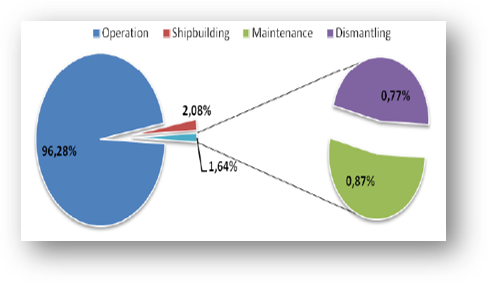
\includegraphics[width= \linewidth]{report-fig/shipbuilding_pie.png}
		\caption{Full life cycle vessel GHG emissions analysis}
		\label{fig:shipbuilding_pie}
	\end{minipage}
	\begin{minipage}[t]{0.49\textwidth}
		\centering
		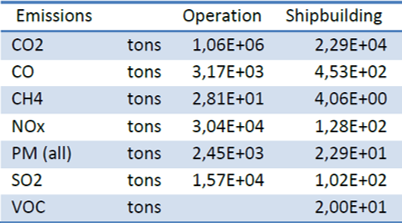
\includegraphics[width=\linewidth]{report-fig/shipbuilding table.png}
		\caption{Absolute GHG emission values}
		\label{fig:shipbuilding_table}
	\end{minipage}
\end{figure}

Finally, for ship i, its GHG emission in shipbuilding phase are given by:
\begin{equation}
	GHG_{building,i} = \dfrac{DWT_i}{74926} * 2290 \, \text{tons}
	\label{eq:shipbuilding}
\end{equation}

\paragraph{Elasticity between freight rate and supply:}
In figure \ref{fig:elasticity}, we give the specific calculation of the elasticity 1.93 in equation (\ref{eq:fr_mf}).\\

\begin{figure}[htbp]
	\centering
	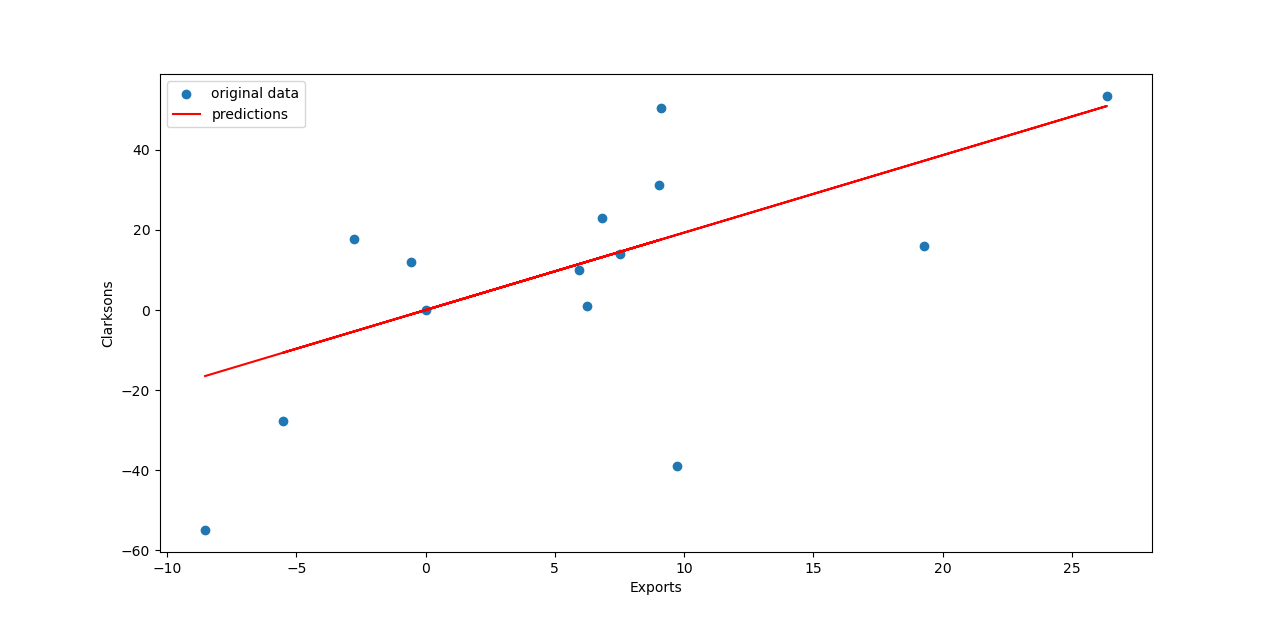
\includegraphics[width=0.5\linewidth]{report-fig/Elasticity.png}
	\caption{Linear relationship between the Clarkson Freight Index and Chinese exports}
	\label{fig:elasticity}
\end{figure}

The Clarkson Index is provided by Crédit Agricole while the China exports data comes from \href{https://fred.stlouisfed.org/series/XTEXVA01CNM667S}{[FRED]}.
All raw data are calculated by month.
Before performing a linear regression, we first calculate an annual average of the data.
This has two advantages, one of which is that it removes the effect of periodicity within each year.
The second is that the overall fluctuations for a year (-10\% to +30\%) are greater than for a month (-5\% to +5\%) and the resulting elasticity can be applied more widely, therefore more reliable.

\paragraph{Parameters in Competition Model:} In the Competition model, the main parameters we need to evaluate are $a, b, l, \gamma, x, \lambda$.

$a,b$ are parameters in the price formula:

\begin{equation*}
	p(u) = a - b \frac{1}{N}\sum_{i=1}^N u_i
\end{equation*}

We can calculate $a,b$ by using the elasticity between price and supply:
\begin{equation}
	\label{eq:price_est}
	p = p_0  - a \dfrac{u-u_0}{u_0} p_0 = 2.93 p_0 - 1.93 \dfrac{p_0}{u_0}u
\end{equation}
where $p_0 = FR \cdot 95\% \cdot Capacity \cdot T * u_0 / D$, $T = 365 \cdot 24 = 8760 h$, D is the voyage distance of route chosen and $u_0$ is the original equilibrium speed in equation (\ref{eq:u0}).

By comparing equation (\ref{eq:price}) with (\ref{eq:price_est}), we can obtain:

\begin{equation}
	a = 5p_0, \quad b = 4 \dfrac{p_0}{u_0}
\end{equation}

And $l, \gamma$ are parameters in the price formula:
\begin{equation*}
	c(u_i) = l u_i + \frac{1}{2 \gamma} u_i^2
\end{equation*}

By definition, the above equation can be rewritten as the sum of operational cost and the fuel cost. By comparing with equations (\ref{eq:operation_cost}) and (\ref{eq:fuel_consumption}) we get
\begin{equation}
	l = OC \cdot \dfrac{T}{D}, \quad \gamma = \dfrac{u_0^2}{2\cdot FC(u_0)}
\end{equation}

Finally, we need to estimate the $x$ and $\lambda$ in equation (\ref{eq:y}):
\begin{equation*}
	y_i = x_i + \lambda(u_i-u_0)
\end{equation*}

To solve this problem, we need to translate the CII policy into a linear version under the assumption that the fuel cost per nautical mile is linearly related to speed.
We start with a linear version formula of CII calculation:
\begin{equation}
	\label{eq:cii_linear}
	CII(\delta) = CII_0\cdot (\dfrac{u_0+\delta}{u_0})=CII_0\cdot (1 + \dfrac{\delta}{u_0})
\end{equation}

Thus,

\begin{equation}
	\delta = \left( \dfrac{CII(\delta)}{CII_0} -1 \right) \cdot u_0
\end{equation}

Note the boundary of the CII E rating as $CII_E$.
Then, different ships will have different maximum acceleration limits $\delta_{max}$, i.e. not exceeding the maximum speed available strictly under the E rating, because of the different $CII_0$ at the same initial speed $u_0$. The $\delta_{max}$ can be calculated by:
\begin{equation}
	\delta_{max,i} = \left( \dfrac{CII_E}{CII_{0,i}} -1 \right) \cdot u_0
\end{equation}

Here we get different ships from the same starting point $u_0$, with different acceleration limits.
But $x$ in equation (\ref{eq:y}) is a different departure point. In order to translate different upper limits of acceleration at the same initial speed into different initial values of x at the same upper $\theta$, we can go to an abstract $\theta_0$ and define $x$ as:
\begin{equation}
	x_i = \theta_0 - \delta_{max,i}
\end{equation}

\subsubsection{Optimal choice to maximize 4-year profit}

In Global Emission Control model, two main parts involve intensive calculations.
The first part focuses on finding the optimal solution for a vessel between the years 2023-2026, taking into account CII (Carbon Intensity Indicator) limits as described in section 2.2.2, equation ({\ref{eq:vast}}).
To solve this problem, the calculations were performed using the NumPy library in Python.
By utilizing \texttt{numpy.argmax}, the best choice among all possible combinations of speeds could be determined.\\

The NumPy library in Python is well-suited for such calculations as it provides efficient numerical operations on arrays and matrices.
Its extensive range of mathematical functions and operations allows for the optimization of vessel speeds and the evaluation of profitability.
By systematically evaluating all speed combinations, the configuration that maximizes profit while adhering to the specified CII limits can be identified.
More precisely, the \texttt{numpy.argmax} function does not aim to find an optimal solution in the traditional algorithmic sense. Instead, it is a simple utility function designed to efficiently retrieve the index of the maximum value(s) in a NumPy array.
The algorithm used by \texttt{numpy.argmax} is straightforward and can be summarized as follows:

\begin{enumerate}
	\item The function initializes the maximum value (\texttt{max\_value}) to a very small value (e.g., negative infinity) and the index of the maximum value (\texttt{max\_index}) to zero.
	\item It iterates over each element in the array, comparing it with the current \texttt{max\_value}. If the element is greater than the current \texttt{max\_value}, it updates \texttt{max\_value} to the new maximum and \texttt{max\_index} to the index of the element.
	\item After iterating over all the elements, it returns \texttt{max\_index} as the index of the maximum value in the array.
\end{enumerate}

It's important to note that the purpose of \texttt{numpy.argmax} is not to find the optimal solution in terms of algorithmic complexity or performance optimization.
Instead, it provides a convenient way to obtain the indices of maximum values in an array using highly optimized NumPy routines, which leverage low-level optimizations for efficient array manipulation and element-wise comparisons.\\



There could be 'smarter' solutions like reverse order calculation.
Indeed, the main problem with the reverse order algorithm in section 2.2.2 lies in the emergence of the DDD situation. This problem can probably be improved by specialized treatment of the DDD case.
For example, when the optimal option for 2023-2025 is CDD and the maximum profit rate for 2023 leads to an CII of D, different combinations of C and D can be tried, e.g. DCD, DCC. However, the validity of this improved algorithm has yet to be tested and proved mathematically.
For the moment, using the full calculation to find the maximum value takes two seconds per ship and is therefore not the most urgent part to improve.\\


\subsubsection{EM Algorithm}

The second part of intensive calculations of the report involves calculating an equilibrium point for flexible prices, as outlined in section 2.2.4 and 2.3.
To address this problem, the classic EM (Expectation-Maximization) algorithm was employed.
The EM algorithm is an iterative optimization technique commonly used in statistics and machine learning to estimate parameters in probabilistic models with latent variables.\\

% The EM algorithm offers several advantages. Firstly, it facilitates the handling of cases where certain variables or data points are unobserved or missing (in this model, we don't have a very precise prevision for future freight rates).
% By iteratively estimating the hidden or latent variables, the EM algorithm provides a principled approach to dealing with incomplete data.
% Secondly, the algorithm usually guarantees convergence to a local optimum, ensuring that a stable solution is obtained even when starting from an initial guess.
% This property proves useful in finding equilibrium points in economic models, as in this case.\\

% However, the EM algorithm also has certain limitations. One limitation is its sensitivity to the choice of initial parameters or starting points.
% Depending on the initial conditions, the EM algorithm may converge to different local optima, potentially leading to different results.
% It is important to be aware of this and consider running the algorithm multiple times with different initialization conditions to mitigate this issue.
% But in our case it is difficult because the initial market condition are prefixed by forward contracts and futures.\\

However, the EM algorithm can be computationally demanding.
The iterative nature of the algorithm requires repeating certain steps until convergence, which can be time-consuming for complex problems.
Therefore, it is crucial to optimize the implementation and take into account the available computational resources.
In our case, the main job is to choose a balanced tolerance, so that we can get close to the optimal solution within reasonable time.
For a given market, such as the container ship market, we set the condition that the set of four-year velocities for all $n$ container ships has an average absolute error of less than $0.025$ relative to the previous iteration.
This condition can be expressed as:
\begin{equation}
	\frac{1}{n}\sum_{i=1}^{n} \frac{1}{4} \sum_{t=1}^{4} \left| \text{velocity}_{i,t} - \text{previous\_velocity}_{i,t} \right| < 0.025
\end{equation}

In this formula, the variables and terms represent the following:
\begin{itemize}
	\item $n$ is the total number of container ships in the market.
	\item $\text{velocity}_{i,t}$ represents the velocity of container ship $i$ in year $t$.
	\item $\text{previous\_velocity}_{i,t}$ represents the velocity of the same container ship $i$ in the previous iteration.
\end{itemize}

And for Competition model, the only change is that there is only one year.\\

In summary, the NumPy library in Python was used to efficiently calculate the profitability of different vessel speeds while considering CII limits.
For the calculation of equilibrium points with flexible prices, the EM algorithm was employed, which offers advantages such as handling missing data and converging to local optima.
However, it is important to consider the sensitivity to initial conditions and the computational demands of the EM algorithm.\\







\subsection{Results}
% Present the quantitative results of your experiments. Graphical data presentation such as graphs and histograms are frequently better than tables.
\subsubsection{Results of Global Emission Control Model}
\paragraph{Annual Profit Maximization}
We start with Step 1, where the year chosen is 2023. Detailed information on the route and fuel consumption, speed etc. can be seen in table \ref{table:comparison}.


\begin{table}[ht]
	\caption{Comparison of Key Metrics for Container Ship 01 and Bulker 01}
	\centering
	\begin{tabular}{l|l|l}
		\hline
		\textbf{Metric}            & \textbf{Container Ships}  & \textbf{Bulkers} \\
		\hline
		Type                       & Post Panamax < 10 000 TEU & Capesize \& VLOC \\
		Capacity                   & 9115 TEU                  & 181336 DWT       \\
		Route                      & Shanghai-Rotterdam        & Houston-Shanghai \\
		Distance (nm)              & 11999.0                   & 12324.0          \\
		Freight Rate               & \$1000.0/TEU              & \$35.0/DWT       \\
		Carbon Tax                 & \$0.0/ton                 & \$0.0/ton        \\
		Utilization                & 95.0\%                    & 90.0\%           \\
		Retrofit                   & False                     & False            \\
		2021 Speed (knots)         & 16.45                     & 12.07            \\
		Optimal Speed 2023 (knots) & 15.30                     & 12.76            \\
		Fuel cost                  & \$-143.51/TEU             & \$-7.25/DWT      \\
		Operation cost             & \$-178.46/TEU             & \$-6.49/DWT      \\
		Profitability              & 65.80\%                   & 60.73\%          \\
		Annual Profit (M\$)        & 39.94                     & 20.74            \\
		Speed Variation            & -7.01\%                   & +5.69\%          \\
		Emission Variation         & -23.16\%                  & +16.03\%         \\
		2021 CII class             & D                         & C                \\
		Current CII class          & B                         & D                \\
		\hline
	\end{tabular}
	\label{table:comparison}
\end{table}

\begin{figure}[htbp]
	\centering
	\begin{minipage}[t]{0.49\textwidth}
		\centering
		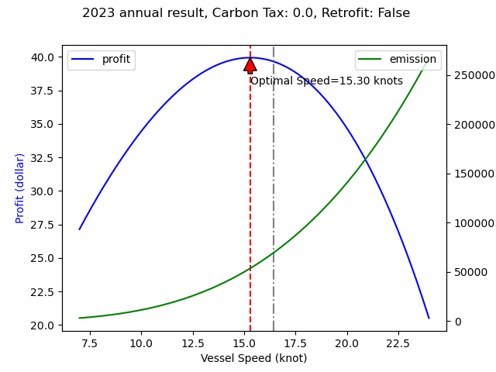
\includegraphics[width= \linewidth]{report-fig/container01.png}
		\caption{Annual Profit Maximization of Container Ship 01}
		\label{fig:container01}
	\end{minipage}
	\begin{minipage}[t]{0.49\textwidth}
		\centering
		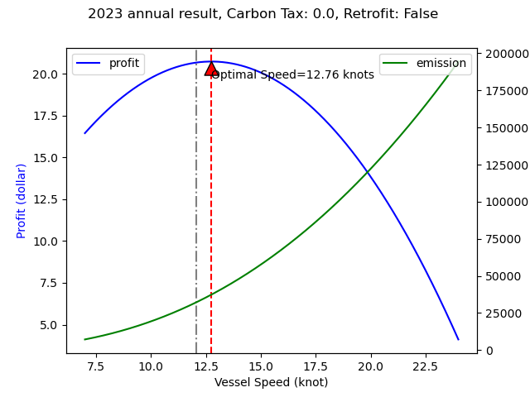
\includegraphics[width= \linewidth]{report-fig/bulker01.png}
		\caption{Annual Profit Maximization of Bulker 01}
		\label{fig:bulker01}
	\end{minipage}
\end{figure}


\subsubsection{Results of Competition Model}


\subsection{Discussion}
% Is your hypothesis supported? What conclusions do the results support about the strengths and weaknesses of your method compared to other methods? How can the results be explained in terms of the underlying properties of the algorithm.


\section{Conclusion}
\end{document}
